\section{Materials and Methods}
\subsection{Data sources and cohort characteristics}
\label{sec:dataset}
We used the processed intestinal tissue RNA-seq count matrices compiled for TENTACLES \cite{montesi2026tentacles}; we did not reprocess raw sequencing reads. The collection contains 689 samples labelled CD (495) or \emph{Not IBD} (194), grouped into four analytical cohorts from six BioProjects (Table~\ref{tab:cohorts}). The comparison label is retained from the source data, but does not imply that every control was a healthy volunteer. For instance, D3 includes non-tumour intestinal tissue from colorectal-cancer surgery \cite{friedrich2021il1}.

\begin{table}[!t]
\caption{Cohort composition by source BioProject.}
\label{tab:cohorts}
\centering\footnotesize
\setlength{\tabcolsep}{3.5pt}
\renewcommand{\arraystretch}{1.1}
\begin{tabular}{@{}llrrr@{}}
\toprule
Cohort & BioProject(s) & $n$ & CD & Not IBD\\
\midrule
D1 & PRJNA248469 & 260 & 218 & 42\\
D2 & \shortstack[l]{PRJNA565216\\PRJNA985602} & 179 & 134 & 45\\
D3 & PRJNA702434 & 76 & 34 & 42\\
D4 & \shortstack[l]{PRJNA728646\\PRJNA961704} & 174 & 109 & 65\\
\midrule
Total & Six BioProjects & 689 & 495 & 194\\
\bottomrule
\end{tabular}
\end{table}

The CD fraction ranges from 44.7\% (D3) to 83.8\% (D1), and median assigned counts across common genes range from 1.78 to 12.01 million per sample. The cohorts also differ in tissue site: D1 comprises ileal biopsies; D2 includes ileal and colonic biopsies; D3 includes small- and large-intestinal samples; and D4 does not provide tissue-site labels in the supplied metadata. Source count CSVs lacked sample identifiers and had 670 rows ordered differently from their metadata. We recovered the IDs from accompanying R data files, aligned expression rows to metadata and verified the original counts and labels without changing their values. The original matrices contained 10,061 genes for D1--D3 and 41,257 for D4; the shared gene-name intersection contained 9,983 genes.

Seven D3 records carried exclusion flags from the source study's quality-control assessment \cite{friedrich2021il1}. They were retained to match the published 76-sample D3 cohort; their inclusion remains a limitation. Exploratory principal-component analysis (PCA) shows cohort-associated expression structure (Fig.~\ref{fig:pca}). It does not establish whether the differences are technical or biological and was not used to train models.

\begin{figure}[!t]
\centering
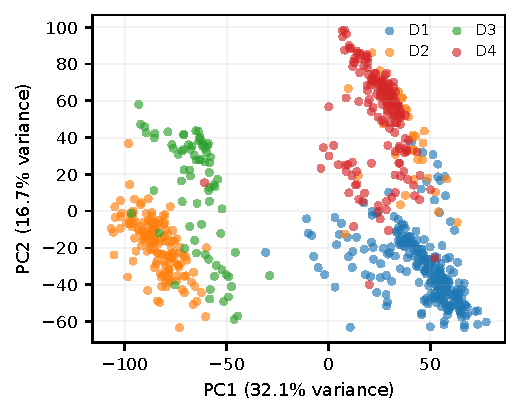
\includegraphics[width=\columnwidth]{cohort_pca_ieee.pdf}
\caption{Exploratory PCA of $\log_2(1+\mathrm{CPM})$ expression across shared genes, coloured by cohort. This descriptive visualisation was not used in model fitting.}
\label{fig:pca}
\end{figure}
